\documentclass[a4paper,10pt]{article}
\usepackage[margin=0.8cm]{geometry}
\usepackage[utf8]{inputenc}
\usepackage{hyperref}
\usepackage{url}
\usepackage{graphicx}
\usepackage{pbox}


\newcommand{\negspace}{\!\!\!}
\newcommand{\idp}{\perp \negspace \perp}
\newcommand{\nidp}{\not \idp}
\newcommand{\dep}{\top \negspace \top}
\newcommand{\ndep}{\not \dep}
\newcommand{\ra}{\rightarrow}

%opening
\title{Uncertainty in Artificial Intelligence - Cheat sheet}
\author{Dieter Castel \& Pierre Carbonnelle}

\begin{document}

\maketitle


\section{General Probability}

$$\begin{array}{l|c}
    \textrm{ Formula} & \textrm{Comment}  \\ 
    p(x,y,z) = p(x \wedge y \wedge z) = p(x,z|y)p(y) & \textrm{Joint Probability Distribution (JPD)}\\
    \\
    p(x \vee y) = p(x) + p(y) - p(x \wedge y) & \textrm{Disjunction for probabilities} \\
    \\
    p(x|y) = \frac{p(x,y)}{p(y)} = \frac{p(y|x)p(x)}{p(y)} & \textrm{definition of Conditional Probablity Dist. (CPD)}\\
    \\
    p(\neg x) = 1-p(x) & \textrm{only valid for probability distributions i.e. normalized!} \\
    \\
    p(x) = \sum_{x,z} p(x,y,z) & \textrm{marginalisation} \\
    \\
    \sum_{y,z} p(x|y,z) = 1 & \textrm{marginalisation of CPD sums to one.} \\
    \\
    size(p(\hat{x},\hat{y},\hat{z})) = \#dom(\hat{x})*\#dom(\hat{y})*\#dom(\hat{z}) & \textrm{\textbf{without} independence assumptions} \\
    \\
    p(x_1,\ldots,x_n) = p(x_1)p(x_2|x_1)p(x_3|x_2,x_1) \ldots p(x_k|x_{k+1},\ldots,x_{n}) & \textrm{Chain rule}  \\ 
  \end{array}
$$

Scientific inference:
$$ \textrm{Posterior distribution} = p(\Theta| D ) = \frac{ p(D|\Theta) p(\Theta) }{ \int_{\Theta} p(D|\Theta)p(\Theta)} = \frac{\textrm{generative Model * Prior}}{\textrm{Normalization Constant} (= Z)} = \frac{\mathrm{likelihood * prior} }{\textrm{evidence}} $$ 

$$\begin{array}{l|c}
    \textbf{ Point Estimates: \hfill Model $M$, Data $D$ and Parameters $\Theta$} & \textrm{Name \hfill (ABRV, comment)}  \\ 
    \\
     \Theta_{\*ML} = argmax_{\Theta} p( D | \Theta, M) = argmax_{\Theta} p( \Theta, D | M)  & \textrm{Maximum Likelihood \hfill  (ML)} \\
     & ( discrete + fully obsv. = just counting) \\
     \Theta_{\*MAP} = argmax_{\Theta} p( \Theta | D, M) = argmax_{\Theta} p(D|\Theta,M)p(\Theta|M)  & \textrm{Maximum A Postiori \hfill (MAP, )} \\
     \\
     \Theta_{\*MoP} = \langle p( \Theta | D, M) \rangle & \textrm{Mean of Postiori \hfill (MoP)} \\
  \end{array}
$$
\section{Distributional Independence}

$$\begin{array}{l|c}
    \textrm{ Formula} & \textrm{Comment}  \\ 
    X \idp Y \iff  \forall x \in X, y \in Y : p(x,y) = p(x)p(y) & \textrm{marginal distributional independence for variable sets X,Y} \\
    \\
    X \idp Y \iff  \forall x \in X, y \in Y: p(x|y) = p(x) & \textrm{marginal distributional independence with CPD def.}\\
    \\
    X \idp Y | Z \iff  \forall x \in X, y \in Y : p(x|y,z) = p(x|z) & \textrm{conditional distributional independence.}\\
  \end{array}
$$

Below is the markov blanket of $x_4$: parents, childeren and parents of its childeren.
\begin{figure}[htb!]
\centering
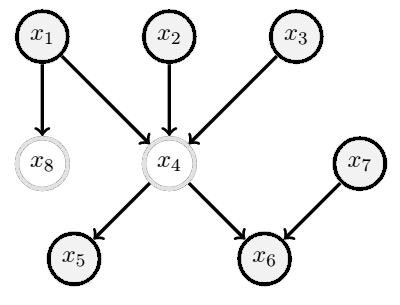
\includegraphics[scale=0.3]{gmarkovblanky.png}
\end{figure}

\newpage
\section{Graphical Independence/d-separation}
In this section $\idp$ and the like only mean GRAPHICAL (in)dependence, \textbf{BEWARE}:\\
\begin{flushright}
(d-separation, $\idp, \ndep$ ==)  Graphical independence $\Rightarrow$ distributional independence. \\
(d-connected, $\nidp,\dep$ ==)  Graphical dependence $\not \Rightarrow$ distributional dependence. 
\end{flushright}




\begin{figure}[htb!]
\begin{tabular}{l||r}
\textbf{colliders} in BN & \textbf{non-colliders} in BN \\
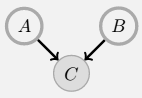
\includegraphics{gcollider.png} & 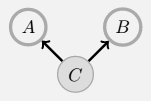
\includegraphics{gnocol.png}  \\
 \large $ A \nidp B | C$ or $ A \dep B | C$ & \large $ A \idp B | C$ or $ A \ndep B | C$ \\
\end{tabular}
\centering
\end{figure}

\subsection{Path-blocking} 
$$\forall p \in allpaths(x,y): blocked(p,Z) \rightarrow isDSeparated(x,y) $$
$$\exists p \in allpaths(x,y): infoflows(p,Z) \rightarrow isDConnected(x,y) $$

A path $p$ is $blocked(p) \iff (1) \vee (2)$
\begin{figure}[htb!]
\begin{tabular}{l||r}
 (1) COLLIDER  & NON-COLLIDER (2) \\
   & $u>v>w$ \\
  $u>v<w$  & $u<v<w$ \\
   & $u<v>w$ \\
$\exists v \in p \setminus \{x,y\} :$ &  $\exists v \in p \setminus \{x,y\} :$ \\
$collider(v) \wedge v \notin Z \wedge descendants(v) \notin Z$  &  $noncollider(v) \wedge v \in Z$\\
colliders and descendants in $Z$ lead to upward info flow. & non-colliders equivalent w.r.t. independence\\
\end{tabular}
\centering
\end{figure}
(d-separation see p43 BRML.)

\subsection{AMDS on complete graph at once} 
Quickest way is with graph edits \textbf{AMDS}. For variable sets $X,Y,Z : X \idp Y | Z$
\begin{enumerate}
 \item \textbf{Ancestral} graph (keep X,Y,Z and ancestors(X,Y,Z)) \hfill \textbf{A}
 \item \textbf{Moralize} (add edges between all parents of the same node) ($\forall v \in A marry(parents(v))$) \hfill \textbf{M}
 \item \textbf{Disorient} (remove arrows) \hfill \textbf{D}
 \item \textbf{Separate} (remove all edges from nodes in Z) \hfill \textbf{S}
\end{enumerate}
\textbf{In the final S graph all unconnected nodes are D-separated.}

\section{Independence Identities}
$$\begin{array}{c|c|c|c}
\textbf{symmetry} & \textbf{decomposition} & \textbf{weak union} & \textbf{contraction} \\
A \idp B | C &  A \idp B,C &  A \idp B,C & A \idp B \wedge A \idp C | B \\
\iff &  \Downarrow & \Downarrow & \Downarrow \\
B \idp A | C &  A \idp B \wedge A \idp C & A \idp B | C \wedge A \idp C | B &  A \idp B,D \\
\end{array}$$

Graphical networks are \textbf{Markov Equivalent} $\iff$ same independencies $\iff$ same skeleton $\wedge$ same immoralities.

$L_p$ set of independencies in JPD $P$.
$L_G$ set of independencies in graph.

\begin{tabular}{l||r}
 I-map (all independencies hold)  & D-Map (all dependencies hold) \\
 $L_g \subseteq L_p$ &  $L_p \subseteq L_g$ \\
 \textbf{EXCLUSION:} Look for an independence in $L_g \notin L_p$ & \textbf{EXCLUSION:} Look for independence in $L_p \notin L_g$ \\
 $\Rightarrow NOT$ I-map & $\Rightarrow NOT$ D-map \\
\end{tabular}

\section{General Inference}

\section{Hidden Markov Models (HMM)}
$$\begin{array}{l|c}
    \textrm{ Formula} & \textrm{Comment}  \\ 
    \\
    p(v_{1:t}, h_{1:t}) = p(h_1) * \Pi^{t}_{i=2} p(v_t|h_t) p(h_t| h_{t-1}) & \textrm{JPD for an HMM}
    \\
    p(v_t | h_t) (= p(v_1 | h_1) \iff \textrm{stationary HMM})   & \textrm{emission matrix} \\
    \\
    \forall t p(v_t | h_t) = p(v_1 | h_1)    & \textrm{emission matrix for stationary HMM} \\
    \\
    p(h_t | h_{t-1})  & \textrm{transmission matrix}  \\
    \\
     & \textrm{ Inference in HMMS} \\
    p(h_t | v_{1:t}) & \textrm{ Filtering (infer up to t)} \\
    \\
    p(h_t | v_{1:T}) (T > t) & \textrm{ Smoothing (use future too)} \\
    \\
    argmax_{h_1:T} p(h_{1:T} | v_{1:T}) & \textrm{ Viterbi (most likely state)} \\
    \\
  \end{array}
$$

\section{Sum-Product on Factor Graphs} 

Singly connected variant BRML p.81.
Loopy? Remove problematic node $R$, SP over new graph, finally: sum/max over the states of removed node $R$.

\begin{figure}[htb!]
\begin{tabular}{l||r}
\textbf{Variable-to-Factor} & \textbf{Factor to Variable} \\
The set $F$ are all factors in the image & The set $V$ are all variables in the image.\\
\\
 $\mu_{v \ra f}(v) = \Pi_{f_i \in F\setminus{f}} \mu_{f_i \ra v}(v) $ & $\mu_{f \ra v}(v) = \sum_{v_i \in V \setminus v} f(v_1,\ldots,v_i, v) \Pi_{y \in \{ne(f) \setminus x\}}$ \\
 product of all factors, $func(v)$ & sum-product over non-$v$ variables, $func(v)$  \\
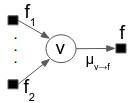
\includegraphics{Var2Fac.png} & 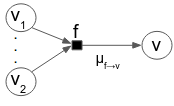
\includegraphics{Fac2Var.png}  \\
 V2Factor = ONLY \textbf{FACTORS} & F2Variable = \textbf{Sum/Max/Argmax AND FACTORS} \\
 $\mu_{v \ra f}(v)$ is a function of $v$ & $\mu_{f \ra v}(v)$ is a function of $v$ \\
 Leaf Factors $= f_i(v)$ & Leaf Variables $= 1$ \\
\end{tabular}
\centering
\end{figure}

\begin{enumerate}
 \item Make factor graph
 \item Pick Root node.
 \item Set leafs (Leaf factor = factor, Leaf Variable = 1)
 \item Propagate messages until required value is computed (up till root for marg inference, backtracking for argmax)
\end{enumerate}

\section{Bucket Elimination}

To calculate $p(x_k)$ from $p(x_1,\ldots,x_k,\ldots,x_n)$:
\begin{enumerate}
 \item Pick and ordering ending with $x_k$
 \item Set all buckets to 1 distribute all factors in order to the buckets 
 \item Eliminate top to bottom: $\sum_v p(v|x_i,\ldots,x_j) = 1$ or redistribute summed bucket to first remaining bucket.
 \item Final bucket is required marginal and still a function of that variable. 
\end{enumerate}

Don't sum over evidential variable.


\section{Distributions }

Beta distribution = 'conjugate' of binomial dist. and conjugate of Beta dist. p.183 BRML; More about Beta Dist see p. 173 BRML

$$\begin{array}{l|c}
 \textrm{formula} & \textrm{comment}\\
\textrm{prior}: B(\alpha,\beta), x \in {0,1} \Rightarrow \textrm{posterior} = B(\alpha + \#^x_1, \beta + \#^x_0) & \textrm{Posterior  with  with Beta-disribution for binary variable $x$}\\
\end{array}$$

\section{Partially Observable Data - Learning with hidden variables}
As opposed to fully observable data. Strategy depends on \textbf{missingness assumptions}. Direction between the visible variables $v_{vis}^i \in x_{vis} = x_{obs}$ and $h_{inv}^i \in x_{inv}$ below is irrelevant.

\begin{figure}[htb!]
\begin{tabular}{l||c||r}
\textbf{Missing Completely At Random} (MCAR) & \textbf{Missing At Random} MAR & \textbf{Missing Not At Random} (MNAR) \\
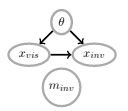
\includegraphics{gMCAR.png} & 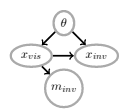
\includegraphics{gMAR.png} & 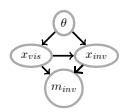
\includegraphics{gMNAR.png}  \\
$x_i \idp m_i$ & $x_i \idp m_i | x_{vis}$ & $x_i \dep m_i$ \\ 
marginal idp between var. & Conditional idp between var. &  dependence between var. \\
and its missingness var. & and its missingness var.   &  and its missingness. \\ 
& $\sum_{h_i} \ldots = \sum_{x_{inv}} \ldots $ couples vars. & \textbf{NON-identifiable} \\ \hline \\ 
 $\Downarrow$ & $\Downarrow$ \textbf{LEARNING SOLUTION} $\Downarrow$ &  $\Downarrow$ \\
Delete samples with missing data & $m_i$ factored out + sol. 4 coupling = & \textit{(out of scope of UAI)} \\  
\& regular $\Theta_*ML$/... &  Expectation Maximisation (EM) & Requires EXTRA assumptions \\ 
%slide 19-22 lecture 8 
\end{tabular}
\centering
\end{figure}

\section{Expectation Maximisation}

Learning method under MAR assumption \textbf{guaranteed} to converge.

\begin{enumerate}
 \item guess $\Theta^0$ (n=0 start with uniform distributions or randomly)
 \item until convergence$(\Theta^{n-1},\Theta^{n})$ do: \\
       \textbf{E}: compute $\forall i,k : q^i_{k} = p(h^i=values(k) | v^i, D, \Theta^{n-1})$ \hfill $\Theta^{n-1}$-weighted estimate of (completed) data for all missing var. \\
       \textbf{M}: compute $\Theta_*ML$ given E by weighted counting. \hfill Probabilistic counting using $q^i_k$'s from \textbf{E}\\
       $n += 1$
\end{enumerate}


\section{sampling}
%TODO


\section{Importance ''sampling'' = approximate averaging}

Calculates $\langle f(x) \rangle_{p(x)}$ given a known importance distribution $q(x)$ ($S_q$ are samples of $q(x)$) \& evaluable function $p*(x)$ such that $p(x) = p*(x)/Z$ and    : 
$$ \langle f(x) \rangle_{p(x)} = \sum_{x^l \in S_q} f(x^l) w(x^l) \textrm{ where } w^l = w(x^l) = \frac{p^*(x^l)/q(x^l)}{\sum_{x^l} p^*(x^l)/q(x^l)} \textrm{ and } \sum_{x_l} w^l = 1$$

\section{soft and unreliable evidence}
%TODO?




\section{global/local semantics}
%TODO include slide 27-28?


















































\appendix


\section{\LaTeX commands}
%TODO: listing from file included at beginning of document?
Go over all tex files see what sticks.
\section{Credits}


Original google docs by P. Carbonelle to be found here:\\ \url{https://docs.google.com/presentation/d/1sP-PJmo-pW4epfLQs3zoveZGceqw59pPeNAY9OM6dl8/edit#slide=id.p}

Some images taken from the Bayesian Reasoning and Machine Learning book. Found on this URL: \url{http://www.cs.ucl.ac.uk/staff/d.barber/brml/}





















\end{document}
